\documentclass[11pt,a4paper]{article}
\usepackage[a4paper,margin=0.78in]{geometry}
\usepackage{amsmath,amssymb,amsfonts}
\usepackage{graphicx}
\usepackage{booktabs}
\usepackage{array}
\usepackage{tabularx}
\usepackage{multirow}
\usepackage{float}
\usepackage{subcaption}
\usepackage{xcolor}
\usepackage{enumitem}
\usepackage{microtype}
\usepackage{url}
\usepackage[hidelinks]{hyperref}
\usepackage[numbers,sort&compress]{natbib}
\usepackage{caption}
\captionsetup{font=small,labelfont=bf}
\setlength{\parindent}{0pt}
\setlength{\parskip}{5pt}
\renewcommand{\arraystretch}{1.12}

\title{\textbf{Graph-Based Information Propagation and Temporal Learning in a Directed Indian Political Twitter Network}}
\author{\textbf{Nikhil A S}\\MSc Data Science\\Digital University Kerala, Kerala, India\\\texttt{nikhilas.ds25@duk.ac.in}}
\date{October 2026}

\begin{document}
\maketitle

\begin{abstract}
This paper studies information propagation and weekly orientation forecasting in a directed Indian political Twitter network. The working data contain 85,495 tweets and 109,443 supplied directed edges. After user matching, the largest weakly connected component contains 17,598 users and 29,715 edges. The network is sparse, weakly reciprocal, and has a largest strongly connected component of only 17 users, making directed reachability a central constraint on diffusion. The original symmetric propagation setting is shown to be seed-dominated; broader sweeps demonstrate that simulated outcomes depend on transmission asymmetry and seed balance rather than supporting an unconditional dominance claim. To recover temporal structure absent from the supplied edge file, interactions were reconstructed from tweet text, producing 129,604 timestamped events across 109,219 unique directed pairs. The reconstructed pairs cover 99.86\% of the supplied edge set and their counts correlate strongly with the supplied weights. These events form 25 weekly dynamic graph snapshots. In leakage-controlled rolling-origin forecasting over 15 test weeks, persistence remains a strong benchmark. Graph message passing improves over matched feature-only models in some settings, but history-aware graph attention does not improve over a history-plus-structure MLP. The results favor a restrained conclusion: network structure carries measurable signal, while recent behavioral history is the more reliable predictor in this data set.
\end{abstract}

\section{Introduction}
Online political discussion is shaped by both network structure and repeated user behavior. A message can only travel along available interaction paths, yet the chance that a user expresses a similar orientation again may also be strongly influenced by that user's own recent history. Treating these two mechanisms as interchangeable can make a graph model appear more informative than it really is.

This study examines both mechanisms in a directed Indian political Twitter network. It began with a competitive diffusion formulation motivated by earlier work on sentiment-aware information spreading \citep{sharma2026}, but the final analysis is broader. It asks whether the supplied directed topology can sustain meaningful simulated propagation, whether competition changes when transmission and seeding are asymmetric, and whether graph learning adds predictive value once simple temporal baselines are taken seriously.

Three issues are central. First, the graph is weakly connected but only weakly strongly connected, so directed reachability is much smaller than a casual reading of the WCC size would suggest. Second, the supplied binary Target field is closely associated with lexical polarity but is not independently verified sentiment, misinformation, or stance ground truth. Third, the supplied network has no edge timestamps. Temporal edges were therefore reconstructed from visible user references in tweet text and checked against the supplied weighted graph before weekly forecasting was attempted.

The resulting study is organized around three research questions:
\begin{enumerate}[label=\textbf{RQ\arabic*:},leftmargin=16mm]
\item Which structural properties of the directed network constrain potential information reach?
\item How do transmission strength, direction, seed balance, and class asymmetry affect simulated propagation?
\item In weekly rolling-origin forecasting, does graph message passing add value beyond persistence and other node-only history baselines?
\end{enumerate}

The contribution is therefore empirical and methodological rather than architectural. The paper combines directed-network diagnostics, controlled diffusion experiments, temporal-edge reconstruction, leakage-controlled weekly evaluation, matched graph-versus-feature controls, and uncertainty estimates. The main result is conditional rather than promotional: graph structure contains useful information, but greater model complexity does not automatically improve forecasting when recent user history is already available.

\section{Related Work and Positioning}
Epidemic and rumor models provide a long-standing language for describing adoption, transmission, and cessation of spreading \citep{kermack1927,daley1964}. Network diffusion models such as independent cascade and linear threshold formulations make propagation explicitly dependent on graph structure \citep{kempe2003}, while competitive models and misinformation-limitation work consider multiple processes that contend for the same population \citep{shir2016,budak2011,lu2024}. Message-passing analyses further show how transmissibility and network topology jointly determine reachable outbreaks on sparse graphs \citep{karrer2010}.

The present simulation is closest in spirit to Sharma et al. \citep{sharma2026}, who combine sentiment-aware competition, structural influence terms, and temporal graph learning. The current work does not claim to reproduce their setting. It uses a different public Twitter data set, a strongly asymmetric directed graph, and an operational binary orientation label whose semantics require separate validation. This distinction matters because equal transmission and equal seeding can make balanced outcomes a property of the model design rather than an empirical observation.

For representation learning, GCNs aggregate information over graph neighborhoods \citep{kipf2017}; GraphSAGE extends neighborhood aggregation to an inductive setting \citep{hamilton2017}; and GAT learns attention weights over neighbors \citep{velickovic2018}. Temporal graph methods such as EvolveGCN, TGAT, TGN, and JODIE incorporate changing graph structure or interaction time in different ways \citep{pareja2020,xu2020,rossi2020,kumar2019}. Because the supplied edge table has no timestamps, a genuine temporal graph benchmark requires reconstructing time-stamped interactions rather than repeatedly applying a temporal model to one fixed adjacency matrix.

Two methodological principles guide the forecasting part of this paper. First, predictive features for week $t$ must be available strictly before week $t$. Second, a graph model should be compared with a matched feature-only model and with behavioral baselines such as persistence. Without those controls, improved performance cannot be attributed specifically to graph message passing.

\section{Data, Provenance, and Population Construction}
\subsection{Raw tables and provenance}
The working data consist of \texttt{master\_tweets.csv} and \texttt{network\_edges.csv} from the public data release \citep{kaggleipte}. The tweet table contains 85,495 rows with fields Date, User, Tweet, Likes, Retweets, Target, Year, Month, and Day. The network table contains Source, Target, and Weight. Because ``Target'' is also a destination-column name in the edge table, this manuscript refers to the tweet variable as the \emph{orientation label} and to the edge-table destination as the \emph{destination account}.

The public data card reports 85,154 posts, whereas the working tweet file contains 85,495 rows. The reason for the 341-row discrepancy is not documented in the available source material, so it is reported rather than silently reconciled. For reproducibility, SHA-256 checksums of the exact analyzed files are included in Table~\ref{tab:dataaudit}. The semantics of the supplied edge Weight field are also not documented beyond being a numeric interaction-strength value; this paper therefore treats it only as a relative recorded weight and does not infer a specific behavioral meaning such as retweet count, mention count, or follow strength.

\begin{table}[H]
\centering
\small
\caption{Data and population summary. Shares quantify the selection effect introduced by restricting analysis to the largest weakly connected component (WCC).}
\label{tab:dataaudit}
\begin{tabularx}{0.98\textwidth}{@{}l r X@{}}
\toprule
Quantity & Value & Interpretation\\
\midrule
Tweet records & 85,495 & Individual tweet observations\\
Unique tweet users & 58,093 & Accounts represented by at least one tweet\\
Full network nodes & 60,532 & Accounts appearing as Source or destination in the edge table\\
Full directed edges & 109,443 & Supplied weighted Source$\rightarrow$destination relations\\
Matched users & 36,614 & Accounts appearing in both data sources\\
Edges among matched users & 30,774 & Induced directed edge set on the matched population\\
Largest WCC users & 17,598 & 48.06\% of matched users; 30.29\% of tweet-table users\\
Largest WCC edges & 29,715 & 96.56\% of matched-user edges\\
Tweets from WCC users & 37,115 & 43.41\% of all working tweet records\\
Users outside WCC & 19,016 & Mostly isolated after matching; see text\\
Self-loops in WCC & 44 & Reported separately because they do not create new-user reach\\
Observation period & 15 Oct 2022--29 Mar 2023 & Tweet timestamps available; supplied edge timestamps unavailable\\
\bottomrule
\end{tabularx}
\vspace{2mm}
\begin{minipage}{0.96\textwidth}\footnotesize
SHA-256 for the analyzed files:\\ \texttt{master\_tweets.csv}: \path{bb19437507a51f52b785223e41a282af29e4647c4588f2d9e660ce87f0ebb4a9}\\
\texttt{network\_edges.csv}: \path{429eb1bda7bcc887cbd6e724d56cca114d5d92b1e7c2c4a7df1101e8294ed019}.
\end{minipage}
\end{table}

\subsection{Matching and connected-population selection}
User identifiers are matched by exact string equality between the tweet User column and the union of Source and destination accounts in the edge table. The 36,614 matched users are added as nodes before inducing edges, so users with no matched-user edge are retained as isolates during the component audit. This produces 18,081 weak components. The largest contains 17,598 users. Outside it are 19,016 users, of whom 17,375 are isolates; only 1,059 induced edges lie outside the largest WCC. Thus, the population reduction is primarily an isolate-removal effect rather than a choice among many similarly sized connected communities.

Users inside and outside the WCC have the same median tweet count (1 tweet per user). WCC users have 37,115 tweets versus 23,637 tweets for the matched users outside the WCC. Median likes per tweet are 4 inside versus 3 outside, while median retweets are 4 in both groups. These comparisons are descriptive and do not establish representativeness.

\begin{figure}[H]
\centering
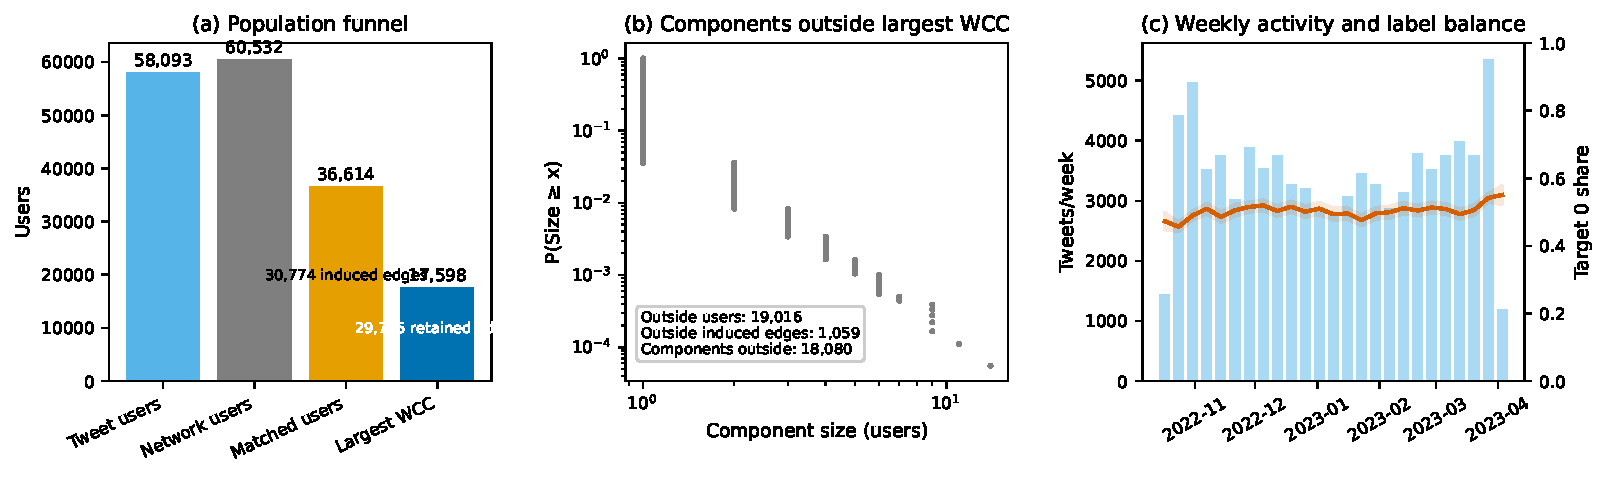
\includegraphics[width=0.98\textwidth]{figures_revised/fig1_study_design_data_funnel.pdf}
\caption{\textbf{Population construction and temporal activity.} (a) User counts from the raw tweet/network sources to the matched set and largest WCC. (b) Component-size CCDF for users outside the largest WCC; most excluded users are isolates. (c) Weekly tweet volume and Target-0 share with Wilson 95\% confidence bands. October and March are partial months.}
\label{fig:funnel}
\end{figure}

\subsection{Reconstructing temporal interactions}
The supplied edge table is static, but the tweet table contains dates and visible user references. A separate reconstruction step therefore extracts three forms of text-visible interaction: retweet patterns of the form ``RT @user'', a leading handle treated as an inferred reply when no native reply metadata are available, and other @mentions. The source is the tweet author and the target is the recovered handle. Usernames are compared case-insensitively and mapped back to the most common spelling found in the supplied network. Within a tweet, a target is counted once, with the priority retweet $>$ inferred reply $>$ mention.

This procedure yields 129,604 timestamped interaction events across 109,219 unique directed pairs. Of these pairs, 109,217 also appear in the supplied network. The precision-style overlap is 99.9982\%, supplied-edge coverage is 99.8638\%, and reconstructed pair counts correlate strongly with the supplied Weight field (Pearson $r=0.9822$; Spearman $\rho=0.9155$). These values show that the text-derived interaction structure closely matches the supplied graph, although they do not establish that the undocumented Weight field is literally a temporal interaction count.

The timestamped events are grouped into Monday-start UTC weeks, producing 25 non-empty weekly snapshots from 10 October 2022 through 27 March 2023. A weekly snapshot contains, on average, 4,083.76 active nodes and 4,994.40 directed edges. Historical node features are calculated from cumulative interactions strictly before the target week and include in-degree, out-degree, in-strength, out-strength, weighted PageRank, and reverse PageRank. The first week has no historical feature rows, and users first appearing in a target week are treated as cold starts rather than being back-filled with future information.

The reconstruction remains an approximation. Leading mentions do not prove native replies, quoted text can obscure attribution, and interactions without visible handles cannot be recovered. The temporal graph is therefore described as a \emph{reconstructed interaction graph}, not platform ground truth.

\section{Orientation-Label Validation Check}
The original project interpreted Target 0 as negative information and Target 1 as positive information after manual inspection of 200 tweets. That interpretation is too strong for the evidence available. To examine the label directly, TextBlob polarity was recomputed for all 85,495 tweet rows \citep{textblob}. Target 0 contains 19,327 lexically negative, 22,652 neutral, and 1,021 positive tweets. Target 1 contains 842 negative, 2,743 neutral, and 38,910 positive tweets. The simple rule $\mathbb{1}[\text{polarity}>0]$ agrees with the supplied Target label for 94.67\% of rows.

This high agreement does \emph{not} prove how the original dataset creator generated Target, but it shows that Target is very close to a positive-versus-non-positive lexical split in the working data. The paper therefore uses the neutral terms \emph{Target 0} and \emph{Target 1} rather than equating them with harmful/beneficial information, misinformation/truth, or verified sentiment. TextBlob is also English-oriented and can miss Hindi, Hinglish, sarcasm, stance, and contextual political meaning; human multilingual annotation remains a required external validation step.

\begin{figure}[H]
\centering
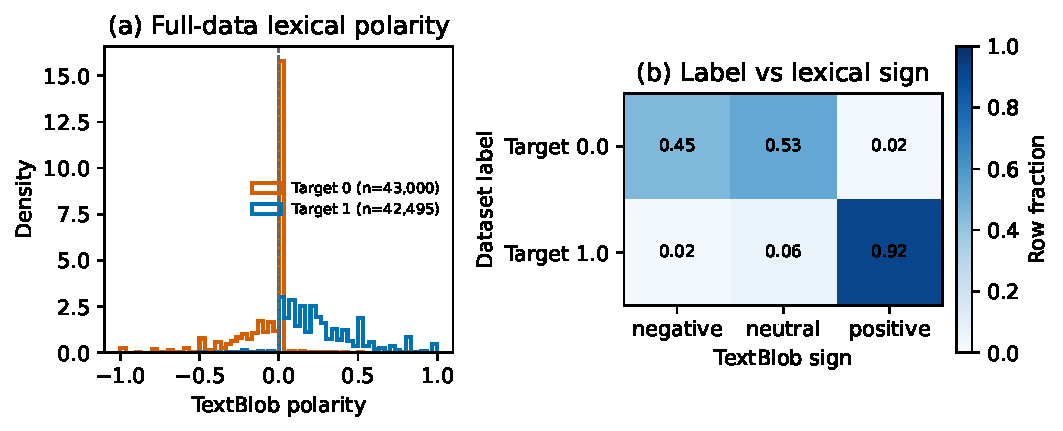
\includegraphics[width=0.82\textwidth]{figures_revised/fig_label_audit_textblob.pdf}
\caption{\textbf{Full-data lexical check of the supplied Target label.} (a) TextBlob polarity distributions for all 85,495 tweets. (b) Row-normalized cross-tabulation of Target against negative/neutral/positive TextBlob sign. The large neutral mass in Target 0 and the 94.67\% agreement with polarity $>0$ for Target 1 motivate treating Target as an operational orientation label rather than independently validated sentiment ground truth.}
\label{fig:labelaudit}
\end{figure}

\section{Directed Network Structure}
The 17,598-user analysis graph is sparse and strongly asymmetric. It contains 29,715 directed edges, density $9.596\times10^{-5}$, reciprocity 0.00936, 17,455 strongly connected components, and a largest strongly connected component (SCC) of only 17 users. Mean out-degree is 1.6885. The supplied edge weights range from 1 to 151, with median 1 and mean 1.209.

The degree and strength distributions are heavy-tailed in the descriptive sense, but this paper does not claim a scale-free law because no formal power-law-vs-lognormal likelihood-ratio fit has been established \citep{clauset2009}. The more important structural observation is directed reachability: relative to the largest SCC, only 172 nodes are in the IN region and 78 in the OUT region, while 17,331 nodes lie in tendril/other structure. A weakly connected graph therefore does not imply broad directed propagation.

\begin{figure}[H]
\centering
\begin{subfigure}[t]{0.49\textwidth}\centering
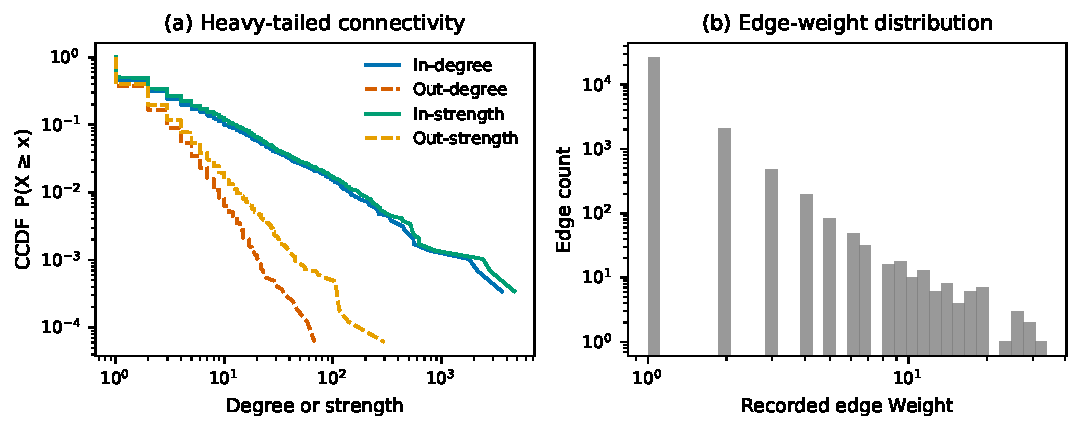
\includegraphics[width=\linewidth]{figures_revised/fig2_network_structure_ccdf.pdf}
\caption{Degree/strength CCDFs and the supplied Weight distribution.}
\end{subfigure}\hfill
\begin{subfigure}[t]{0.49\textwidth}\centering
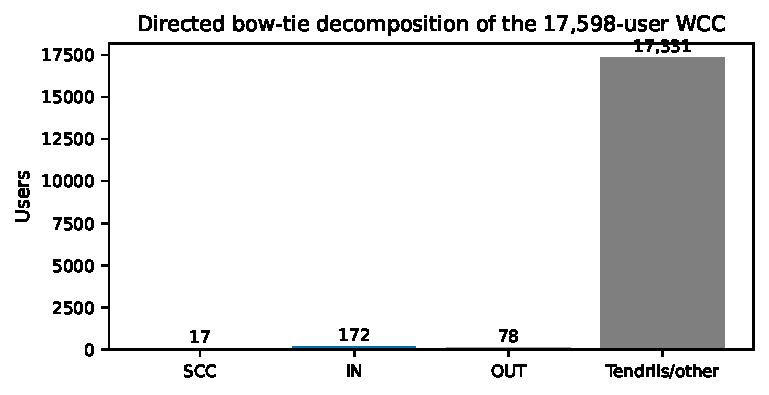
\includegraphics[width=\linewidth]{figures_revised/fig3_bow_tie.pdf}
\caption{Bow-tie decomposition around the 17-node largest SCC.}
\end{subfigure}
\caption{\textbf{The analysis graph is sparse and directionally constrained.} Heavy-tailed connectivity coexists with a very small strongly connected core, limiting the set of nodes mutually reachable by directed paths.}
\label{fig:networkstructure}
\end{figure}

\subsection{Direction-aware structural influence}
The first implementation called $0.6\,D+0.4\,PR$ a ``trust'' score. Because neither degree nor PageRank measures observed credibility, the term \emph{trust} is dropped. In addition, standard PageRank emphasizes incoming prominence, whereas propagation from a source depends on its outgoing relations. The analysis therefore uses source-side out-strength and reverse PageRank.

For each node $i$, let $R_{out}(i)$ be its percentile rank by weighted out-strength and $R_{rPR}(i)$ its percentile rank by PageRank on the reversed graph. The structural-influence score is
\begin{equation}
S_i = 0.6R_{out}(i)+0.4R_{rPR}(i), \qquad S_i\in[0,1].
\end{equation}
The 60/40 weighting remains a modeling choice rather than an estimated optimum. Rank normalization is used to avoid the collapse produced by min--max scaling of strongly skewed centralities.

Spearman correlation between standard and reverse PageRank is $-0.147$, confirming that source-side and sink-side prominence are not interchangeable. A direction-reversal control at a strong transmission setting produced a mean final reach of 319.5 users under the Source$\rightarrow$destination assumption and 373.5 under reversed edges; the paired mean difference was 54 users with a wide 95\% bootstrap interval of $[-24.4,166.8]$. Thus direction affects outcomes, but 40 paired runs do not support a precise directional effect estimate.

\begin{figure}[H]
\centering
\begin{subfigure}[t]{0.49\textwidth}\centering
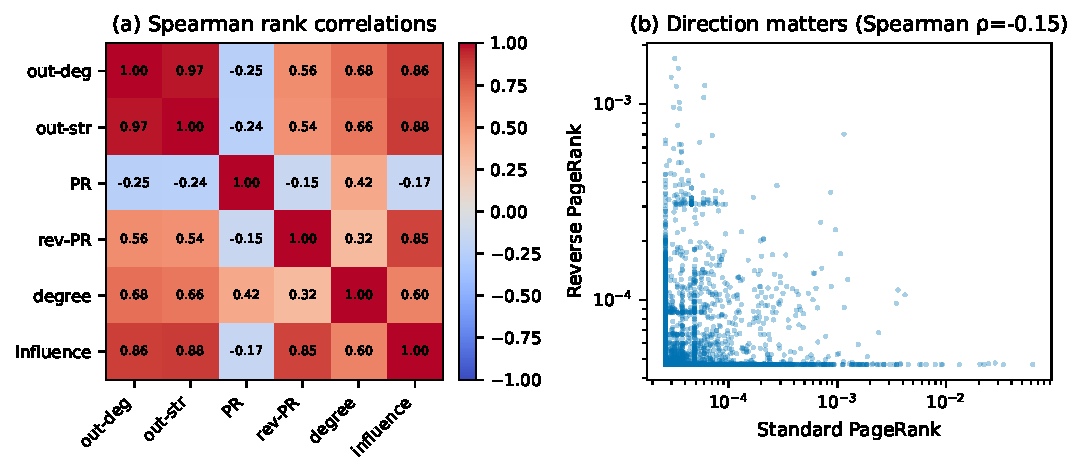
\includegraphics[width=\linewidth]{figures_revised/fig4_centrality_direction.pdf}
\caption{Rank correlations and standard-vs-reverse PageRank.}
\end{subfigure}\hfill
\begin{subfigure}[t]{0.49\textwidth}\centering
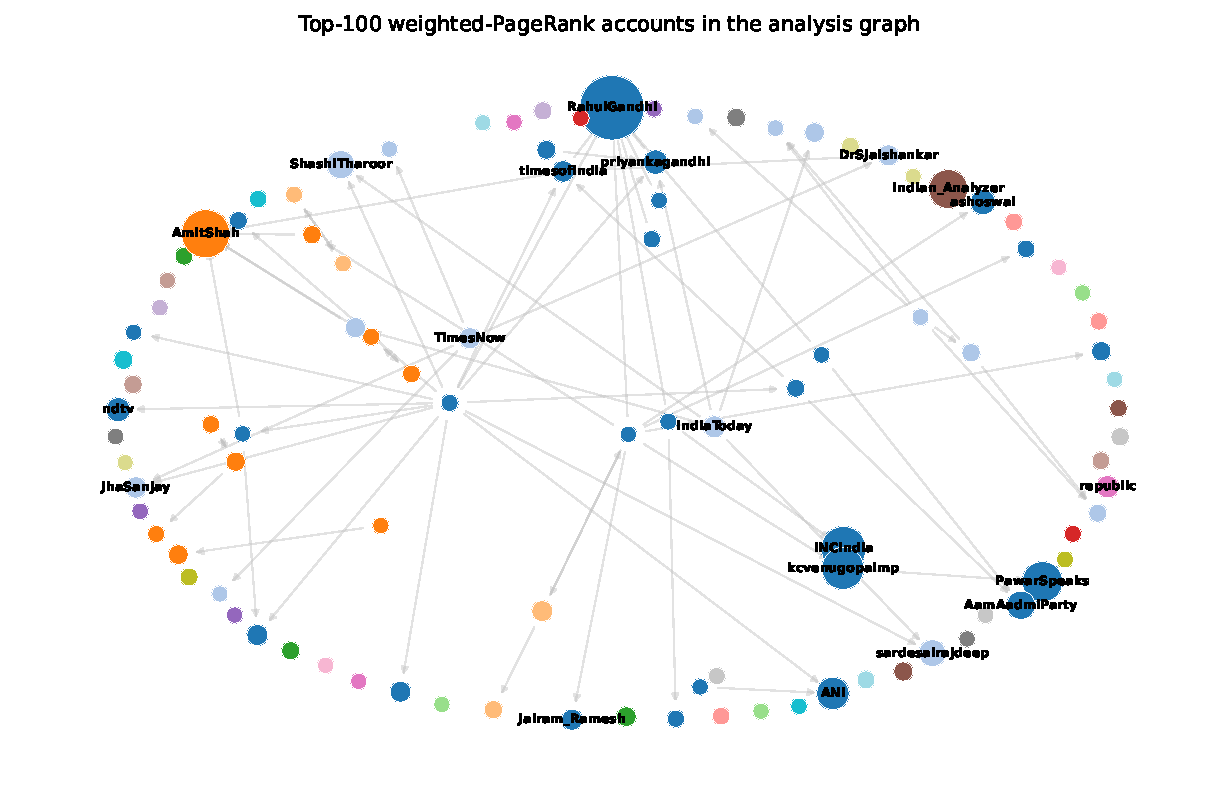
\includegraphics[width=\linewidth]{figures_revised/fig6_top100_pagerank_wcc.pdf}
\caption{Top-100 weighted-PageRank accounts within the 17,598-user WCC.}
\end{subfigure}
\caption{\textbf{Structural prominence depends on edge direction.} The left panel shows that standard PageRank and source-side measures are not equivalent. The right panel is a descriptive visualization: node size reflects weighted PageRank in the WCC and colors are greedy-modularity communities on the top-100 induced subgraph. Public account handles are displayed only as dataset identifiers; no political identity or causal influence is inferred.}
\label{fig:centrality}
\end{figure}

\subsection{Orientation mixing and a label-shuffle null}
For each user, the Target-0 ratio is the fraction of that user's tweets labeled Target 0. Users are descriptively grouped as Target-0 majority ($\geq0.6$), Target-1 majority ($\geq0.6$ Target 1), or mixed. Edge-level mixing is then compared with a null distribution from 500 random permutations of the continuous Target-0 ratios over nodes. The observed source--destination Spearman correlation is 0.0085; the two-sided empirical permutation $p$-value is 0.158. Thus this analysis does not provide evidence of strong orientation homophily beyond random label placement on the fixed graph.

\begin{figure}[H]
\centering
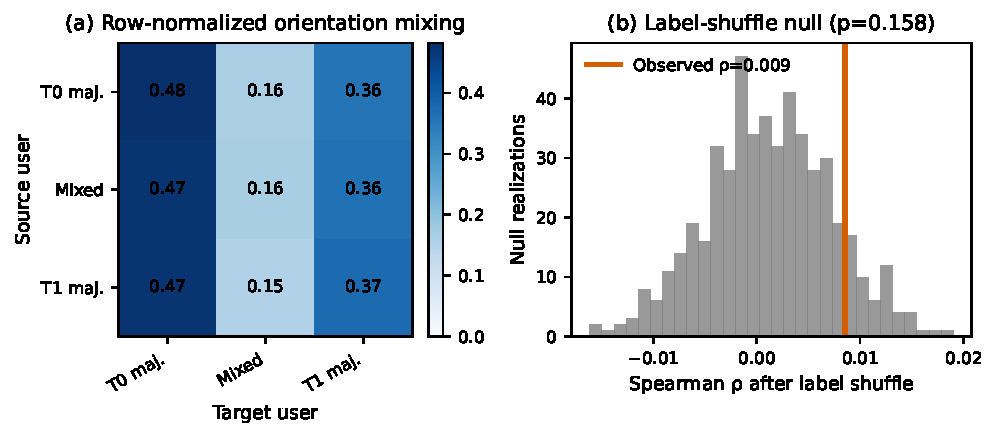
\includegraphics[width=0.82\textwidth]{figures_revised/fig5_orientation_mixing_null.pdf}
\caption{\textbf{Observed orientation mixing is weak.} (a) Row-normalized edge mixing among Target-0-majority, mixed, and Target-1-majority users. (b) Label-shuffle null distribution for source--destination Target-0-ratio correlation; the observed value ($\rho=0.0085$) is not extreme ($p=0.158$).}
\label{fig:mixing}
\end{figure}

\section{Stochastic Propagation Model}
\subsection{States and edge semantics}
The supplied network contains Source, destination, and Weight but does not document whether an edge represents a mention, retweet, follow, or another interaction. The primary simulation treats Source$\rightarrow$destination as the available propagation direction solely as a modeling assumption; the direction-reversal control above quantifies sensitivity to that choice.

To avoid the clinical connotation of ``recovered,'' each node is in one of four states
\begin{equation}
X_i(t)\in\{S,A_0,A_1,Q\},
\end{equation}
where $S$ is susceptible, $A_0$ and $A_1$ are active Target-0- and Target-1-oriented spreaders, and $Q$ is a quiescent absorbing state that has stopped spreading. The model does not allow $A_0\leftrightarrow A_1$ conversion or reactivation from $Q$; those are explicit model limitations.

\subsection{Edge and node modifiers}
The edge factor is
\begin{equation}
f_w(w_{ij})=\frac{\log(1+w_{ij})}{\max_{(u,v)\in E}\log(1+w_{uv})},
\end{equation}
which compresses the 1--151 weight range without applying an ineffective logarithm to tiny PageRank values. Let $r_i^{(k)}$ be user $i$'s overall fraction of tweets with Target class $k\in\{0,1\}$. The class-specific source orientation multiplier is
\begin{equation}
M_k(i)=0.5+0.5r_i^{(k)},
\end{equation}
and the structural multiplier is
\begin{equation}
M_S(i)=0.5+0.5S_i.
\end{equation}
TextBlob does not enter the transmission model; it is used only in the lexical label check in Section~4.

For an active source $i$ and susceptible destination $j$, the one-step transmission probability is
\begin{equation}
p_{ij}^{(k)}=\min\left(1,\;\beta_k f_w(w_{ij})M_S(i)M_k(i)\right).
\label{eq:trans}
\end{equation}
If multiple active sources of class $k$ point to $j$, their exposure probability is aggregated by the complement rule
\begin{equation}
E_j^{(k)}=1-\prod_{i\in\mathcal{N}^{(k)}_j}\left(1-p_{ij}^{(k)}\right),
\end{equation}
where $\mathcal{N}^{(k)}_j$ is the set of currently active class-$k$ in-neighbors of $j$. Independent Bernoulli draws determine whether class-0 and/or class-1 exposure succeeds. If both succeed in the same step, the adopted state is drawn proportionally to $E_j^{(0)}$ and $E_j^{(1)}$. Active nodes stop spreading with probability $\gamma$ after their transmission attempts.

\subsection{Synchronous update order}
Each simulation step uses the following order:
\begin{enumerate}[leftmargin=8mm]
\item compute exposure attempts from nodes active at the start of the step;
\item aggregate multiple class-specific exposures for each susceptible destination;
\item resolve simultaneous class-0/class-1 successes proportionally;
\item draw recovery/quiescence for the previously active nodes;
\item activate newly adopted nodes for the \emph{next} step.
\end{enumerate}
Seeds are counted in final cascade size. Self-loops are ignored for new-user transmission because a node cannot newly infect itself once active.

\section{Threshold, Sensitivity, and Competition Experiments}
\subsection{Why the first simulation was uninformative}
The first implementation used $\beta_0=\beta_1=0.14$, $\gamma=0.25$, and 25 seeds per contagion. Reported final sizes were approximately the seed counts, so the process generated almost no secondary spread. Under the edge and node factors, the spectral radii of the class-specific weighted operators are $\rho_0=0.9163$ and $\rho_1=0.7880$. A linearized threshold diagnostic $\beta_c\approx\gamma/\rho$ gives $\beta_{c,0}\approx0.2728$ and $\beta_{c,1}\approx0.3173$. The old $\beta=0.14$ is below both of these diagnostic thresholds, consistent with seed-dominated cascades. Because the finite directed graph is highly non-strongly-connected, these values are treated as linearized reference points, not exact phase-transition constants.

The phase sweep uses a 1\% seed fraction (176 seeds), 40 independent runs per cell, and $\beta/\beta_c\in\{0.2,0.35,0.5,0.7,0.85,1,1.2,1.5,2,3,5\}$. Reach increases with $\beta$, but it remains structurally constrained: at $5\beta_c$, mean final reach is 310 users for Target 0 and 325 for Target 1 (1.76\% and 1.85\% of the WCC). The result is therefore not a claim of a sharp macroscopic epidemic transition; rather, it demonstrates that the directed topology imposes a hard practical constraint on reach.

\begin{figure}[H]
\centering
\begin{subfigure}[t]{0.49\textwidth}\centering
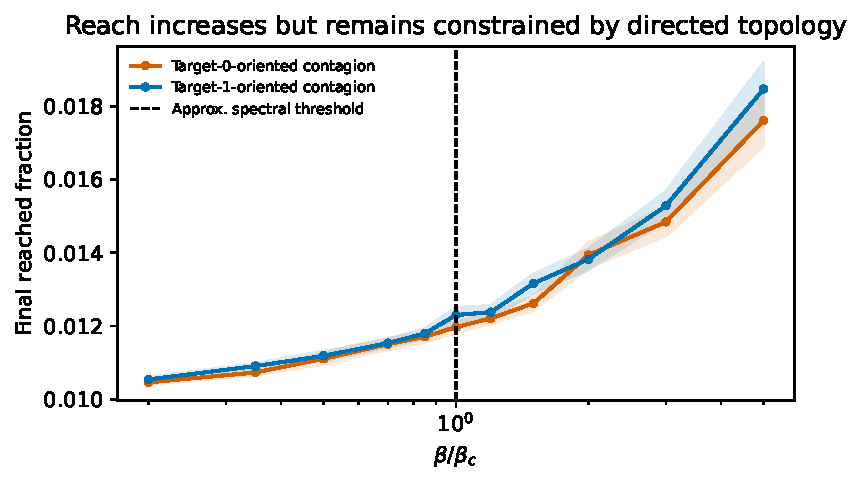
\includegraphics[width=\linewidth]{figures_revised/fig8_phase_transition.pdf}
\caption{Final reached fraction across $\beta/\beta_c$ with 95\% CIs over 40 runs.}
\end{subfigure}\hfill
\begin{subfigure}[t]{0.49\textwidth}\centering
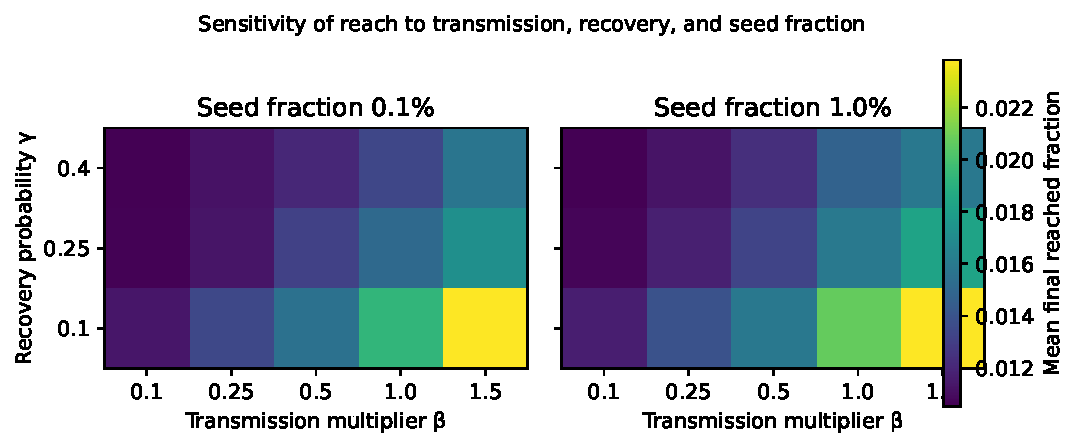
\includegraphics[width=\linewidth]{figures_revised/fig_sensitivity_grid.pdf}
\caption{Sensitivity to transmission, recovery, and seed fraction (20 runs/cell).}
\end{subfigure}
\caption{\textbf{Reach increases with transmission but remains limited by directed structure.} Higher $\beta$, lower $\gamma$, and more seeds increase reach; even strong transmission does not produce a population-wide cascade on this WCC.}
\label{fig:threshold}
\end{figure}

\subsection{Competition is controlled by asymmetry and seed balance}
The earlier conclusion that neither class ``dominates'' was not a valid empirical finding because the model used equal transmission, equal recovery, and symmetric seeding. The competition experiment varies both the transmission ratio and the seed share. The outcome statistic is
\begin{equation}
\Delta=\frac{C_0-C_1}{C_0+C_1},
\end{equation}
where $C_0$ and $C_1$ are final reached counts. A total seed budget of 1\% of nodes is split between classes, $\log_{10}(\beta_0/\beta_1)$ ranges from $-1$ to $1$, and 20 runs are averaged per grid cell.

The outcome map shows the expected falsifiable pattern: larger Target-0 transmission or a larger Target-0 seed share shifts $\Delta$ positive, while the opposite asymmetry favors Target 1. Near equal transmission and equal seed share, the mean outcome is close to zero. Symmetric parity is therefore a \emph{model property}, not evidence that real political information types spread equally.

\begin{figure}[H]
\centering
\begin{subfigure}[t]{0.49\textwidth}\centering
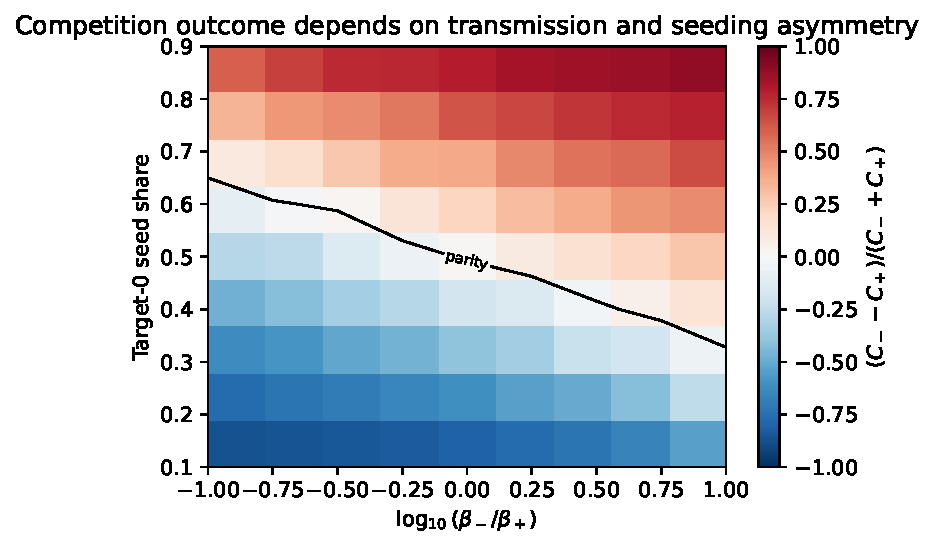
\includegraphics[width=\linewidth]{figures_revised/fig9_competition_outcome_map.pdf}
\caption{Outcome map over transmission ratio and Target-0 seed share.}
\end{subfigure}\hfill
\begin{subfigure}[t]{0.49\textwidth}\centering
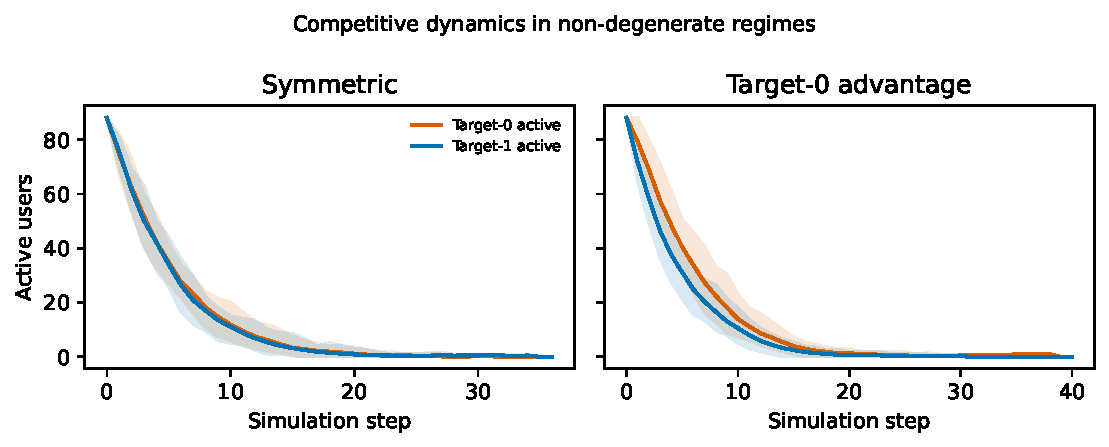
\includegraphics[width=\linewidth]{figures_revised/fig10_compartment_time_series.pdf}
\caption{Active-state trajectories for symmetric and Target-0-favored settings.}
\end{subfigure}
\caption{\textbf{Competition outcomes depend on explicit asymmetry.} The parity contour moves with both transmission and seed balance, showing why an equal-parameter baseline cannot test a dominance hypothesis. Bands in the time-series panels show the 5th--95th percentile range over 30 runs.}
\label{fig:competition}
\end{figure}

\section{Mean-Preserving Component Controls}
The original ablation replaced normalized edge weights by one, which simultaneously removed structure and increased the average transmission scale. To separate those effects, the controls preserve mean per-edge transmission while changing only the association between components and edges/nodes. A strong-transmission setting ($\beta=1.5$, $\gamma=0.25$, 1\% seeds) is used with 40 paired random seeds. Weight shuffling preserves the weight distribution, structural-influence flattening replaces the source multiplier by its edge-weighted mean, orientation flattening replaces orientation by its mean, and orientation shuffling permutes node orientation while preserving its distribution.

\begin{table}[H]
\centering
\small
\caption{Mean-preserving component controls. Effects are paired differences in final reached users relative to the full model; 95\% CIs are bootstrap intervals over 40 paired runs.}
\label{tab:ablation}
\begin{tabular}{lrrr}
\toprule
Variant & Mean final size & $\Delta$ vs full & 95\% CI for $\Delta$\\
\midrule
Full model & 321.45 & 0.00 & --\\
Weight shuffled & 321.20 & -0.25 & [-8.80, 8.55]\\
Structural influence flattened & 312.53 & -8.93 & [-19.20, 0.60]\\
Orientation flattened & 321.60 & 0.15 & [-8.45, 8.48]\\
Orientation shuffled & 318.53 & -2.93 & [-11.10, 5.98]\\
\bottomrule
\end{tabular}
\end{table}

None of the intervals excludes zero. The earlier claim that edge weights were the ``largest contributor'' is therefore removed. The valid conclusion is narrower: changing the \emph{scale} of edge transmission had a large effect in the old ablation, but shuffling weight structure while preserving mean transmission does not show a reliable effect in this 40-run control.

\section{Leakage-Controlled Weekly Forecasting}
\subsection{Prediction cohort and rolling-origin protocol}
Weekly user labels are constructed from tweets occurring within each Monday-start UTC week. For each user-week, Target-0 and Target-1 counts are compared; ties are left unlabeled and excluded from binary evaluation. This produces 77,247 user-week label records, including 1,500 ties. A prediction row is retained only when the user has a non-tied label for the target week and a historical graph-feature row computed strictly before that week. The final prediction data set contains 16,292 user-week records. A further 59,455 labeled user-weeks lack the required historical graph features and are excluded from the primary evaluation; these exclusions include both first-appearance cold starts and users who had tweeted previously without entering the reconstructed interaction graph.

Forecasting uses 15 rolling test weeks from 19 December 2022 through 27 March 2023. For each test week, the immediately preceding eligible week is used for validation and all earlier eligible weeks form the training set, subject to a minimum eight-week training history. Numeric scaling and class weighting are fitted on training data only. Hyperparameters are chosen on validation data only, and the test week is used once for evaluation. Users may reappear across weeks because the task is future behavior forecasting for previously observed users rather than user-disjoint generalization.

The first comparison includes a training-majority classifier, persistence, logistic regression, a multilayer perceptron (MLP), and a gated recurrent unit (GRU). Persistence predicts the most recent non-tied prior orientation for a user, with a training-prevalence fallback when no earlier label exists. Logistic regression and the MLP use six structural features: in/out degree, in/out strength, PageRank, and reverse PageRank. The GRU uses sequences of historical structural features. Neural models are repeated with ten seeds (42--51).

\begin{table}[H]
\centering
\small
\caption{Weekly rolling-origin baseline performance across 15 test weeks. Class-0 average precision is reported against the class-0 prevalence reference for each week.}
\label{tab:weeklybaselines}
\begin{tabular}{lrrr}
\toprule
Model & Mean macro-F1 & Mean class-0 AP & Mean balanced accuracy\\
\midrule
Majority & 0.3460 & 0.5292 & 0.5000\\
Persistence & \textbf{0.5396} & \textbf{0.5575} & \textbf{0.5403}\\
Logistic regression & 0.4742 & 0.5529 & 0.5121\\
MLP & 0.4522 & 0.5494 & 0.5066\\
GRU & 0.4487 & 0.5464 & 0.5055\\
\bottomrule
\end{tabular}
\end{table}

Persistence is the strongest of these baselines. The GRU does not establish a benefit over the MLP: paired confidence intervals for the predeclared comparison metrics include zero, and the GRU exceeds Persistence in macro-F1 in only one of the 15 test weeks. Structural features still carry some signal---for example, logistic regression exceeds the majority baseline in macro-F1 in all 15 weeks---but temporal feature sequences alone do not provide a reliable gain.

\subsection{Static and temporal graph models}
The graph experiment adds static GCN, GraphSAGE, GAT, and a GRU-over-GCN temporal model. The latter is referred to as \emph{Temporal GCN}; it is not presented as EvolveGCN-O or EvolveGCN-H. All models use the same rolling origins, ten random seeds, training-only preprocessing, and historical cutoffs. Direction controls compare message passing along Source$\rightarrow$destination edges with reversed messages. For GAT and GraphSAGE, reversed direction is evaluated explicitly because incoming prominence and outgoing spreading opportunity need not be equivalent on this network.

Across the graph models, reversed GAT has the highest mean macro-F1, 0.4943. It remains below Persistence by $-0.0453$ macro-F1 (95\% bootstrap CI $[-0.0551,-0.0349]$), but it exceeds the node-only MLP by $+0.0421$ ($[0.0211,0.0640]$). In a matched feature-only control, adding reversed GAT message passing improves macro-F1 by $+0.0231$ ($[0.0135,0.0342]$). Reversed GAT also exceeds the weekly class-0 prevalence reference in average precision in all 15 test weeks. These comparisons indicate that graph neighborhoods contain useful predictive information when the model is restricted to structural features.

The temporal model does not show the same advantage. Temporal GCN minus aligned GRU is $+0.0020$ macro-F1 with a 95\% CI of $[-0.0033,0.0068]$, and Temporal GCN minus the best static graph model is $-0.0047$ with a CI of $[-0.0159,0.0069]$. Neither interval excludes zero. Temporal graph evolution therefore does not provide an established improvement over comparable node-only temporal modeling or the strongest static graph model in this experiment.

Direction affects which aspect of performance is favored. Reversing GAT messages improves macro-F1, while forward messages give better class-0 average precision. The network therefore does not support a single direction-independent notion of ``best'' message passing.

\subsection{Does graph structure add value beyond behavioral history?}
Because Persistence is difficult to beat, a final matched experiment gives learned models access to historical orientation information as well as structural features. The history variables are the most recent prior label, an indicator for whether such a label exists, past class proportions, count of prior labeled weeks, and weeks since the last label. All are computed strictly before the prediction week.

History-only logistic regression obtains the highest mean macro-F1, 0.5529. A history-plus-structural MLP reaches 0.5496, while the matched history-plus-reversed-GAT model reaches 0.5184. The central comparison is therefore negative: GAT minus MLP is $-0.0312$. Its ordinary bootstrap 95\% CI is $[-0.0444,-0.0208]$; moving-block bootstrap intervals are $[-0.0375,-0.0221]$ with three-week blocks and $[-0.0372,-0.0232]$ with four-week blocks. The Holm-adjusted $p$-value is 0.00122. Excluding users without label history yields the same qualitative result.

History-only logistic regression has the best mean macro-F1, but its improvement over Persistence does not survive Holm correction. The history-plus-MLP does improve over Persistence on class-0 average precision, balanced accuracy, and Matthews correlation coefficient. Taken together, these results show that recent behavioral history carries most of the predictive signal available to the tested models. Graph message passing can help when only structural features are available, but it does not add incremental value once historical orientation and structural features are already supplied to the matched MLP.

\begin{figure}[H]
\centering
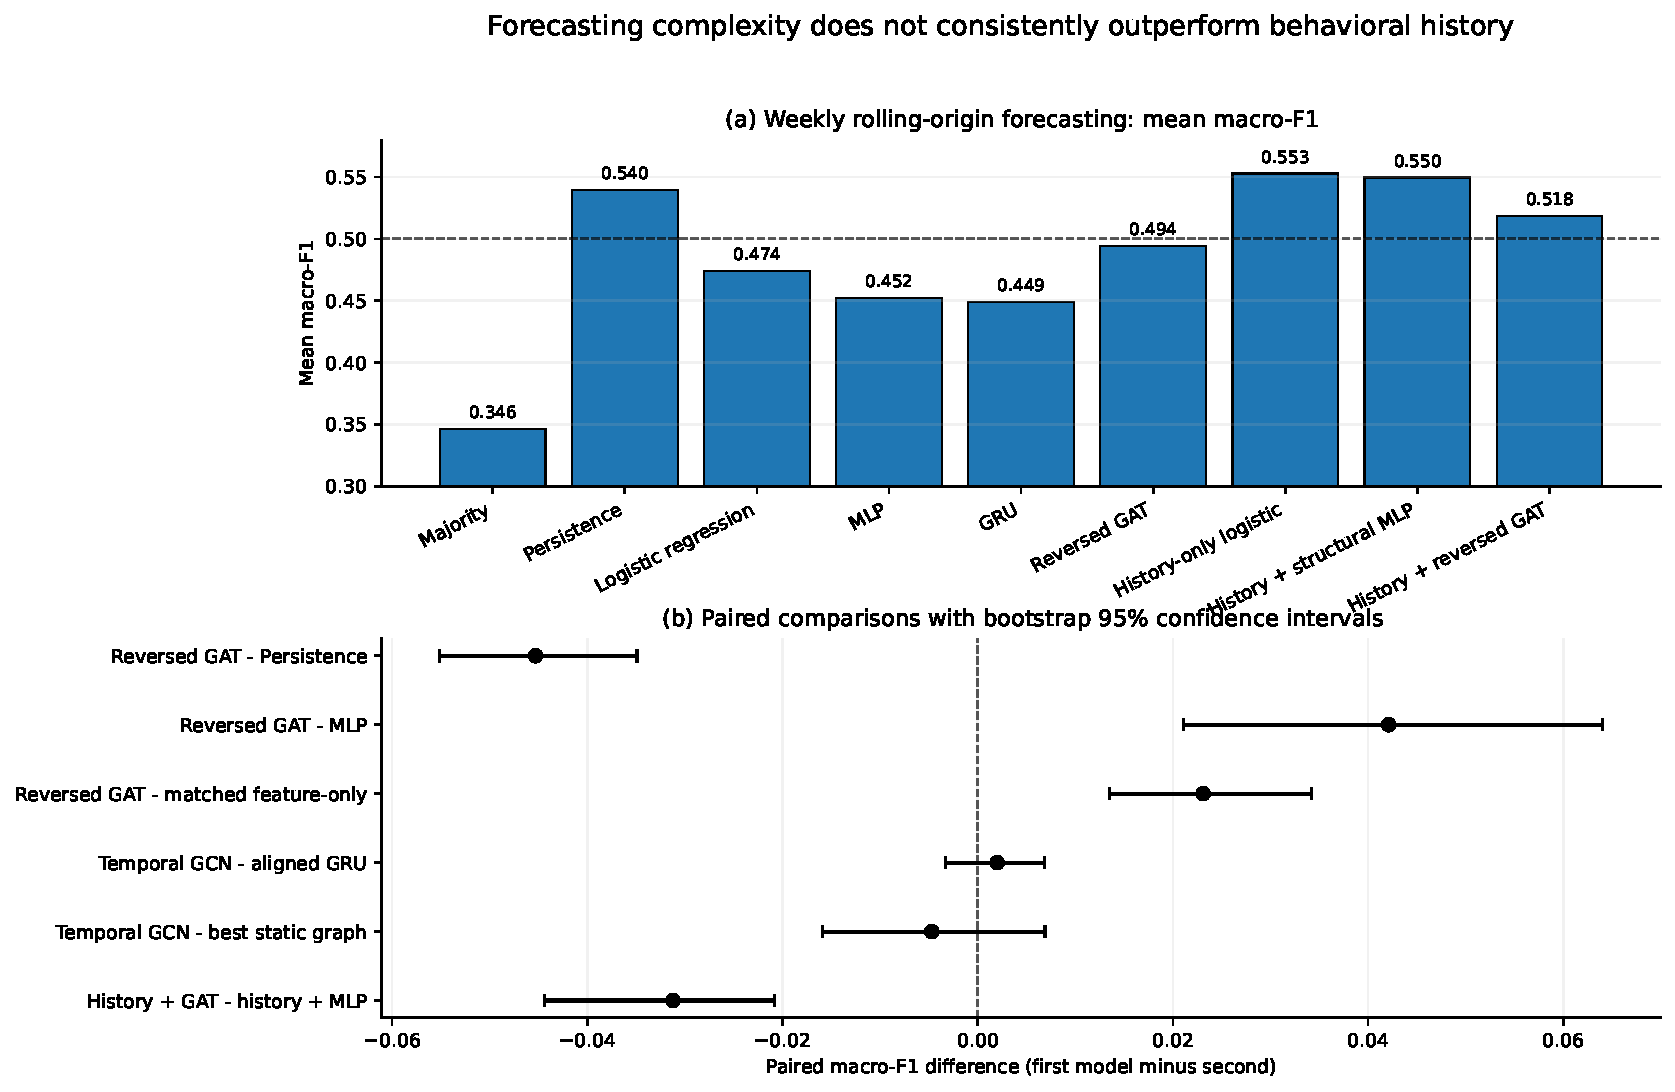
\includegraphics[width=0.97\textwidth]{figures_revised/fig11_weekly_forecasting_summary.pdf}
\caption{\textbf{Forecasting results favor behavioral history over additional graph complexity.} Panel (a) summarizes mean macro-F1 for the main baseline, graph, and history-aware models. Panel (b) shows paired macro-F1 differences with bootstrap 95\% confidence intervals for the central matched comparisons. Positive values favor the first model named in each comparison.}
\label{fig:weeklyforecast}
\end{figure}

\section{Discussion}
The combined structural, simulation, and forecasting results point to a consistent interpretation.

The first point concerns topology. The 17,598-user WCC is not a broadly mutually reachable network: its largest SCC has only 17 users and reciprocity is below 1\%. This is why strong transmission does not automatically generate population-scale cascades. A WCC is useful for defining one connected analysis population, but it should not be treated as evidence that information can flow freely in both directions.

The second point concerns model symmetry. In the original simulation, equal transmission, equal recovery, and symmetric seeding made near-parity unsurprising, while the low transmission scale produced almost no secondary spread. Once transmission and seed balance are varied explicitly, the outcome changes in the expected direction. The appropriate claim is therefore conditional: simulated dominance depends on the chosen asymmetry and the reachable directed structure.

The third point concerns prediction. Reconstructing 129,604 timestamped interactions makes it possible to evaluate genuinely changing weekly graph snapshots rather than a fixed topology with changing node features. The reconstruction agrees closely with the supplied network, which supports its use as a temporal proxy, but it remains text-derived rather than native platform metadata.

The fourth point is that behavioral persistence is a demanding baseline. Reversed GAT outperforms matched feature-only controls when only structural variables are available, so the graph is not irrelevant. However, once recent orientation history is introduced, the matched history-plus-MLP performs better than history-plus-GAT. The final result is therefore not that graph neural networks ``fail''; rather, their incremental contribution is limited after the strongest available non-graph history signal is included.

This distinction matters for model selection. A more complex architecture should be preferred only when it adds reproducible value under the same information boundary. In this data set, the simplest useful summary of the forecasting experiments is that recent user history is more reliable than additional graph complexity, while graph structure provides secondary signal in structurally constrained models.

\section{Limitations}
\begin{enumerate}[leftmargin=7mm]
\item The supplied edge Weight field is undocumented. The strong correlation with reconstructed interaction counts supports a relationship, but does not prove that Weight has one specific behavioral meaning.
\item Temporal edges are reconstructed from visible text cues rather than native interaction metadata. Inferred replies, quoted text, deleted content, and invisible interactions remain sources of error.
\item The supplied Target field is treated as an operational orientation label. TextBlob shows a strong lexical association, but it is not a multilingual human reference standard. A separate multilingual validation is being conducted and is not included in the present results.
\item The forecasting cohort excludes target-week users without historical graph features. Reported results therefore apply to users with usable prior graph history, not all active users.
\item The rolling-origin evaluation contains 15 test weeks. Ordinary bootstrap intervals do not model serial dependence; moving-block intervals improve robustness for the central history-aware comparison but remain approximate with such a short time series.
\item Neural comparisons involve repeated users across weeks. This is appropriate for within-user future forecasting but does not measure performance on entirely unseen users.
\item The GAT implementation uses sampled neighborhoods, and direction controls alter message orientation. Results should therefore be interpreted as model-and-direction specific rather than as universal properties of GAT.
\item The temporal graph model is GRU-over-GCN, not a faithful EvolveGCN-O/H implementation. No claim of EvolveGCN performance is made in the final analysis.
\item Propagation parameters are explored over controlled ranges rather than calibrated from observed adoption cascades. The simulation is a mechanism study, not an estimate of real-world contagion probabilities.
\item Results come from one political Twitter data set. External validity requires a second empirical network or carefully chosen synthetic benchmarks.
\end{enumerate}

\section{Ethics, Data Governance, and Dual Use}
The data concern political discussion and include public account handles. The analysis is restricted to aggregate network structure, supplied orientation labels, and simulation behavior; it does not infer private attributes, ideology, or offline characteristics. Named handles in the top-100 visualization are used only as identifiers already present in the public data source and should not be interpreted as claims about credibility, political identity, or causal influence.

The data source reports a public release, but redistribution of scraped social-media content can still be subject to platform terms. For that reason, the submission package does not redistribute the raw tweet text. It instead provides file checksums, analysis scripts, derived aggregate tables, and figures. Intervention ideas such as blocking or prebunking can have dual-use implications; any future intervention study should evaluate fairness across communities and avoid targeting individuals for political manipulation.

\section{Reproducibility}
All analyses use fixed preprocessing rules and explicit temporal cutoffs. Raw-file hashes are recorded in Table~\ref{tab:dataaudit}. The temporal reconstruction produced 129,604 events with no invalid timestamps, and the weekly graph builder preserved every valid event across 25 snapshots. Forecasting features are based only on interactions strictly before the target Monday; scaling, class weights, and hyperparameter selection are confined to training and validation data.

The baseline and neural experiments use the same 15 rolling test weeks. MLP and GRU models were evaluated over ten random seeds, and the graph experiment used the same seed set. The history-aware matched experiment adds another 600 fits under the same temporal protocol. Bootstrap intervals are paired by test week; the central history-plus-GAT versus history-plus-MLP comparison is additionally checked with three- and four-week moving-block bootstrap intervals and Holm-adjusted tests.

The Overleaf archive contains the manuscript, figures, analysis scripts from the propagation study, and summary tables used in the paper. The seed-level forecasting outputs were generated in the local analysis project and should be deposited with the code and environment specification in any public archival release. No raw tweet text is redistributed in this manuscript package.

\section{Conclusion}
This study began as a graph-diffusion project but ultimately produced a more useful result by testing its assumptions directly. The network is large enough to appear well connected at first glance, yet its directed structure is highly restrictive: the main WCC has a 17-node strongly connected core and very low reciprocity. Simulated spread is therefore governed as much by reachability as by transmission probability, and symmetric competition should not be interpreted as evidence that two information classes behave equally in the real world.

Reconstructing timestamped interactions changes the temporal part of the study substantially. The recovered edge stream closely matches the supplied graph and supports 25 weekly dynamic snapshots. Under a leakage-controlled rolling-origin design, persistence is a strong benchmark, static graph attention adds information relative to matched structural-feature controls, and temporal graph modeling does not show a reliable advantage. Most importantly, once recent orientation history is included, history-plus-GAT performs worse than a matched history-plus-structure MLP. The evidence therefore supports a simple conclusion: network structure is informative, but recent behavioral history is the stronger forecasting signal in this data set.

That conclusion is deliberately narrower than a claim of universal graph-model superiority. Its value lies in showing exactly where structure helps, where complexity does not, and which remaining questions---multilingual label validation, calibrated propagation, native temporal interaction metadata, and cross-data-set replication---must be answered before stronger claims are justified.

\section*{Author Contributions}
Nikhil A S carried out the study design, data preparation, network analysis, simulation, forecasting experiments, visualization, software implementation, and manuscript preparation.

\section*{Funding}
No external funding was reported for this study.

\section*{Competing Interests}
The author declares no competing interests.

\section*{References}
\begin{thebibliography}{99}
\bibitem{sharma2026} A. Sharma, Aishwaraya, B. Mondal, B. F. B. A. Boya, Y. Soula, and S. S. Muni, ``Sentiment-aware competitive graph diffusion model for negative information control in online social networks,'' \emph{Chaos, Solitons \& Fractals}, vol. 209, Art. no. 118535, 2026. doi: 10.1016/j.chaos.2026.118535.
\bibitem{kaggleipte} \emph{Indian Political Tweet Engagement Dataset}, Kaggle public data release, accessed September 2026. The data card reports 85,154 posts; the analyzed working CSV contains 85,495 rows.
\bibitem{kermack1927} W. O. Kermack and A. G. McKendrick, ``A contribution to the mathematical theory of epidemics,'' \emph{Proc. Royal Society A}, vol. 115, no. 772, pp. 700--721, 1927.
\bibitem{daley1964} D. J. Daley and D. G. Kendall, ``Epidemics and rumours,'' \emph{Nature}, vol. 204, p. 1118, 1964.
\bibitem{karrer2010} B. Karrer and M. E. J. Newman, ``Message passing approach for general epidemic models,'' \emph{Physical Review E}, vol. 82, Art. no. 016101, 2010.
\bibitem{kempe2003} D. Kempe, J. Kleinberg, and E. Tardos, ``Maximizing the spread of influence through a social network,'' in \emph{Proc. ACM SIGKDD}, pp. 137--146, 2003.
\bibitem{budak2011} C. Budak, D. Agrawal, and A. El Abbadi, ``Limiting the spread of misinformation in social networks,'' in \emph{Proc. WWW}, 2011.
\bibitem{shir2016} Y. Liu, S.-M. Diao, Y.-X. Zhu, and Q. Liu, ``SHIR competitive information diffusion model for online social media,'' \emph{Physica A}, vol. 461, pp. 543--553, 2016.
\bibitem{lu2024} H. Lu, Y. Wang, and J. Wu, ``An efficient competitive control mechanism for negative information spread in online social networks,'' \emph{Int. J. Bifurcation and Chaos}, vol. 34, no. 14, 2024.
\bibitem{vosoughi2018} S. Vosoughi, D. Roy, and S. Aral, ``The spread of true and false news online,'' \emph{Science}, vol. 359, no. 6380, pp. 1146--1151, 2018.
\bibitem{centola2010} D. Centola, ``The spread of behavior in an online social network experiment,'' \emph{Science}, vol. 329, no. 5996, pp. 1194--1197, 2010.
\bibitem{clauset2009} A. Clauset, C. R. Shalizi, and M. E. J. Newman, ``Power-law distributions in empirical data,'' \emph{SIAM Review}, vol. 51, no. 4, pp. 661--703, 2009.
\bibitem{brin1998} S. Brin and L. Page, ``The anatomy of a large-scale hypertextual Web search engine,'' in \emph{Proc. Seventh International World Wide Web Conference}, pp. 107--117, 1998.
\bibitem{traag2019} V. A. Traag, L. Waltman, and N. J. van Eck, ``From Louvain to Leiden: guaranteeing well-connected communities,'' \emph{Scientific Reports}, vol. 9, Art. no. 5233, 2019.
\bibitem{kipf2017} T. N. Kipf and M. Welling, ``Semi-supervised classification with graph convolutional networks,'' in \emph{ICLR}, 2017.
\bibitem{hamilton2017} W. L. Hamilton, R. Ying, and J. Leskovec, ``Inductive representation learning on large graphs,'' in \emph{Advances in Neural Information Processing Systems}, vol. 30, pp. 1024--1034, 2017.
\bibitem{velickovic2018} P. Veli\v{c}kovi\'c, G. Cucurull, A. Casanova, A. Romero, P. Li\`o, and Y. Bengio, ``Graph attention networks,'' in \emph{ICLR}, 2018.
\bibitem{pareja2020} A. Pareja \emph{et al.}, ``EvolveGCN: Evolving graph convolutional networks for dynamic graphs,'' in \emph{AAAI}, pp. 5363--5370, 2020.
\bibitem{rossi2020} E. Rossi \emph{et al.}, ``Temporal Graph Networks for Deep Learning on Dynamic Graphs,'' arXiv:2006.10637, 2020.
\bibitem{xu2020} D. Xu, C. Ruan, E. Korpeoglu, S. Kumar, and K. Achan, ``Inductive representation learning on temporal graphs,'' in \emph{ICLR}, 2020.
\bibitem{kumar2019} S. Kumar, X. Zhang, and J. Leskovec, ``Predicting dynamic embedding trajectory in temporal interaction networks,'' in \emph{ACM SIGKDD}, pp. 1269--1278, 2019.
\bibitem{textblob} S. Loria, \emph{TextBlob: Simplified Text Processing}, 2018, \url{https://textblob.readthedocs.io/}.
\end{thebibliography}

\end{document}
